%!Mode:: "TeX:UTF-8"
\documentclass[a4paper,11pt,UTF8]{ctexart}
\usepackage{indentfirst} %缩进
\usepackage{xeCJK}    %使用系统字体
\usepackage{fancyhdr} %自定义页眉页脚
\pagestyle{empty}                   %不设置页眉页脚
\usepackage{amsmath, amsthm, amssymb, amsfonts} %数学公式
\usepackage[a4paper,left=3cm,right=3cm,top=3cm,bottom=3cm]{geometry}
%\usepackage[tmargin=1in,bmargin=1in,lmargin=1.25in,rmargin=1.25in]{geometry}.
\usepackage{booktabs} %插入表格
\usepackage[section]{placeins} %避免浮动
\usepackage{listings} %插入代码
\usepackage{ctex}     %中文宏包
\usepackage[svgnames, table]{xcolor} %彩色表格
\usepackage{algorithm}          %伪代码
\usepackage{algorithmicx}
\usepackage{algpseudocode}
\usepackage{algorithm,algpseudocode,float}
\usepackage{lipsum}
\usepackage{enumitem}           %调整列举环境
\usepackage{url}
\usepackage{fontspec,xunicode}
\usepackage{cite}
\defaultfontfeatures{Mapping=tex-text} %如果没有它,会有一些 tex 特殊字符无法正常使用,比如连字符。

\usepackage{graphicx}
\usepackage{subfigure}
\graphicspath{{imgs/}}

%%%%%%%%%%%%%%%%%%%%%%%%%%%%%%%%%%%%%%%%%%%%%%%%%%%%%%%%%%%%%%%%
% 缩进及行间距
%%%%%%%%%%%%%%%%%%%%%%%%%%%%%%%%%%%%%%%%%%%%%%%%%%%%%%%%%%%%%%%%
\setlength{\parindent}{22pt} %重新定义缩进长度
\setlength{\baselineskip}{20pt}  %定义行间距
%\renewcommand{\baselinestretch}{1.1} %定义行间距

%%%%%%%%%%%%%%%%%%%%%%%%%%%%%%%%%%%%%%%%%%%%%%%%%%%%%%%%%%%%%%%%
% 列表设置
%%%%%%%%%%%%%%%%%%%%%%%%%%%%%%%%%%%%%%%%%%%%%%%%%%%%%%%%%%%%%%%%
\setenumerate{fullwidth,itemindent=\parindent,listparindent=\parindent,itemsep=0ex,partopsep=0pt,parsep=0ex}
\setenumerate[2]{label=\alph*),leftmargin=1.5em}  %二级item设置
\setitemize{itemindent=38pt,leftmargin=0pt,itemsep=-0.4ex,listparindent=26pt,partopsep=0pt,parsep=0.5ex,topsep=-0.25ex}
\setdescription{itemindent=38pt,leftmargin=0pt,itemsep=-0.4ex,listparindent=26pt,partopsep=0pt,parsep=0.5ex,topsep=-0.25ex}

%%%%%%%%%%%%%%%%%%%%%%%%%%%%%%%%%%%%%%%%%%%%%%%%%%%%%%%%%%%%%%%%
% 图的标题行间距设置
%%%%%%%%%%%%%%%%%%%%%%%%%%%%%%%%%%%%%%%%%%%%%%%%%%%%%%%%%%%%%%%%
\newcommand{\bottomcaption}{%
\setlength{\abovecaptionskip}{6pt}%
\setlength{\belowcaptionskip}{6pt}%
\caption}


%%%%%%%%%%%%%%%%%%%%%%%%%%%%%%%%%%%%%%%%%%%%%%%%%%%%%%%%%%%%%%%%
% 字体定义
%%%%%%%%%%%%%%%%%%%%%%%%%%%%%%%%%%%%%%%%%%%%%%%%%%%%%%%%%%%%%%%%
\setmainfont{Times New Roman}  %默认英文字体.serif是有衬线字体sans serif无衬线字体
\setmonofont{Consolas}
\setCJKmainfont[ItalicFont={楷体}, BoldFont={黑体}]{宋体}%衬线字体 缺省中文字体为
\setCJKsansfont{黑体}
\punctstyle{hangmobanjiao}
%-----------------------xeCJK下设置中文字体------------------------------%
\setCJKfamilyfont{song}{SimSun}                             %宋体 song
\newcommand{\song}{\CJKfamily{song}}
\setCJKfamilyfont{fs}{FangSong}                      %仿宋  fs
\newcommand{\fs}{\CJKfamily{fs}}
\setCJKfamilyfont{ktgb}{KaiTi}                      %楷体2312 ktgb
\newcommand{\ktgb}{\CJKfamily{ktgb}}
\setCJKfamilyfont{yh}{Microsoft YaHei}                    %微软雅黑 yh
\newcommand{\yh}{\CJKfamily{yh}}
\setCJKfamilyfont{hei}{SimHei}                              %黑体  hei
\newcommand{\hei}{\CJKfamily{hei}}
\setCJKfamilyfont{hwxk}{STXingkai}                                %华文行楷  hwxk
\newcommand{\hwxk}{\CJKfamily{hwxk}}
%------------------------------设置字体大小------------------------%
\newcommand{\shiyanbaogao}{\fontsize{36pt}{\baselineskip}\selectfont}
\newcommand{\chuhao}{\fontsize{42pt}{\baselineskip}\selectfont}     %初号
\newcommand{\xiaochuhao}{\fontsize{36pt}{\baselineskip}\selectfont} %小初号
\newcommand{\yihao}{\fontsize{28pt}{\baselineskip}\selectfont}      %一号
\newcommand{\erhao}{\fontsize{21pt}{\baselineskip}\selectfont}      %二号
\newcommand{\xiaoerhao}{\fontsize{18pt}{\baselineskip}\selectfont}  %小二号
\newcommand{\sanhao}{\fontsize{15.75pt}{\baselineskip}\selectfont}  %三号
\newcommand{\sihao}{\fontsize{14pt}{\baselineskip}\selectfont}       %四号
\newcommand{\xiaosihao}{\fontsize{12pt}{\baselineskip}\selectfont}  %小四号
\newcommand{\wuhao}{\fontsize{10.5pt}{\baselineskip}\selectfont}    %五号
\newcommand{\xiaowuhao}{\fontsize{9pt}{\baselineskip}\selectfont}   %小五号
\newcommand{\liuhao}{\fontsize{7.875pt}{\baselineskip}\selectfont}  %六号
\newcommand{\qihao}{\fontsize{5.25pt}{\baselineskip}\selectfont}    %七号

%%%%%%%%%%%%%%%%%%%%%%%%%%%%%%%%%%%%%%%%%%%%%%%%%%%%%%%%%%%%%%%%
% 图题字体大小相同
%%%%%%%%%%%%%%%%%%%%%%%%%%%%%%%%%%%%%%%%%%%%%%%%%%%%%%%%%%%%%%%%
\usepackage{caption}
\captionsetup{font={footnotesize}}   % footnotesize = 9pt
\captionsetup[lstlisting]{font={footnotesize}}

%%%%%%%%%%%%%%%%%%%%%%%%%%%%%%%%%%%%%%%%%%%%%%%%%%%%%%%%%%%%%%%%
% 重定义枚举编号为 1),2)...
%%%%%%%%%%%%%%%%%%%%%%%%%%%%%%%%%%%%%%%%%%%%%%%%%%%%%%%%%%%%%%%%
\renewcommand{\labelenumi}{\theenumi)}


%%%%%%%%%%%%%%%%%%%%%%%%%%%%%%%%%%%%%%%%%%%%%%%%%%%%%%%%%%%%%%%%
% 重定义section标题
%%%%%%%%%%%%%%%%%%%%%%%%%%%%%%%%%%%%%%%%%%%%%%%%%%%%%%%%%%%%%%%%
\CTEXsetup[format={\sihao\CJKfamily{zhhei}\zihao{4}},number={\chinese{section}},name={,、~},aftername={},indent={0pt},beforeskip={6pt},afterskip={6pt},format+={\flushleft}]{section}
\CTEXsetup[format={\Large\bfseries\CJKfamily{zhkai}\zihao{5}},name={(,)},number={\chinese{subsection}},aftername={},indent={22pt},beforeskip={14pt},afterskip={2pt}]{subsection}
\CTEXsetup[number={\chinese{section}},name={附录, ~~ }]{appendix}



%%%%%%%%%%%%%%%%%%%%%%%%%%%%%%%%%%%%%%%%%%%%%%%%%%%%%%%%%%%%%%%%
% 标题名称中文化
%%%%%%%%%%%%%%%%%%%%%%%%%%%%%%%%%%%%%%%%%%%%%%%%%%%%%%%%%%%%%%%%
\renewcommand\figurename{\hei 图}
\renewcommand\tablename{\hei 表}
\renewcommand\lstlistingname{\hei 代码}
\renewcommand{\algorithmicrequire}{\textbf{输入:}}
\renewcommand{\algorithmicensure}{\textbf{输出:}}
\newtheorem{define}{定义}

%%%%%%%%%%%%%%%%%%%%%%%%%%%%%%%%%%%%%%%%%%%%%%%%%%%%%%%%%%%%%%%%
% 代码设置
%%%%%%%%%%%%%%%%%%%%%%%%%%%%%%%%%%%%%%%%%%%%%%%%%%%%%%%%%%%%%%%%
\lstset{
 columns=fixed,
 numbers=left,                                        % 在左侧显示行号
 numberstyle=\tiny\color{gray},                       % 设定行号格式
 frame=single,                                        % 单线背景边框
 breaklines=true,                                     % 设定LaTeX对过长的代码行进行自动换行
 keywordstyle=\color[RGB]{40,40,255},                 % 设定关键字颜色
 numberstyle=\footnotesize\color{darkgray},
 commentstyle=\it\color[RGB]{0,96,96},                % 设置代码注释的格式
 stringstyle=\rmfamily\slshape\color[RGB]{128,0,0},   % 设置字符串格式
 showstringspaces=false,                              % 不显示字符串中的空格
 language=java,                                        % 设置语言
 basicstyle=\linespread{1.0}\xiaowuhao\ttfamily,                      % 字体字号
 %lineskip=10pt,
 %baselinestretch=1,
}

%%%%%%%%%%%%%%%%%%%%%%%%%%%%%%%%%%%%%%%%%%%%%%%%%%%%%%%%%%%%%%%%
% 伪代码分页
%%%%%%%%%%%%%%%%%%%%%%%%%%%%%%%%%%%%%%%%%%%%%%%%%%%%%%%%%%%%%%%%
\makeatletter
\renewcommand{\ALG@name}{算法}
\newenvironment{breakablealgorithm}
  {% \begin{breakablealgorithm}
   \begin{center}
     \refstepcounter{algorithm}% New algorithm
     \hrule height.8pt depth0pt \kern2pt% \@fs@pre for \@fs@ruled
     \renewcommand{\caption}[2][\relax]{% Make a new \caption
       {\raggedright\textbf{\ALG@name~\thealgorithm} ##2\par}%
       \ifx\relax##1\relax % #1 is \relax
         \addcontentsline{loa}{algorithm}{\protect\numberline{\thealgorithm}##2}%
       \else % #1 is not \relax
         \addcontentsline{loa}{algorithm}{\protect\numberline{\thealgorithm}##1}%
       \fi
       \kern2pt\hrule\kern2pt
     }
  }{% \end{breakablealgorithm}
     \kern2pt\hrule\relax% \@fs@post for \@fs@ruled
   \end{center}
  }
\makeatother



\begin{document}
\xiaosihao\song

\begin{titlepage}
\center{\yihao{\ktgb{中山大学数据科学与计算机学院\\操作系统实验课程}}}
\vspace{1cm}


\center{\shiyanbaogao{\ktgb{实~验~报~告}}}
\vspace{2cm}

\begin{center}
\begin{large}
\begin{tabular}{rc}
\xiaoerhao{\hei{教\qquad 师}}& \sanhao{\hei{凌应标}}\\
\cline{2-2}\\
\xiaoerhao{\hei{学\qquad 号}}& \hspace{1.7cm}\sanhao{\hei{17341035\hspace{1.7cm}}} \\
\cline{2-2}\\
\xiaoerhao{\hei{姓\qquad 名}}& \sanhao{\hei{傅畅}}\\
\cline{2-2}\\
\xiaoerhao{\hei{实验名称}}& \sanhao{\hei{实验六(二状态多进程模型)}}\\
\cline{2-2}\\

\end{tabular}
\end{large}
\end{center}
\vfill \hfill
\end{titlepage}
\clearpage

\centerline{\\[10pt]\erhao{\fs{实~验~六}}}
\centerline{\\[10pt]\yihao{\fs{二~状~态~多~进~程~模~型}}}

\leftline{\\[8pt]\xiaosihao{\hei{\hspace{1.5em} 姓名:傅畅\hfill 学号:17341038 \hfill  }}}

\leftline{\\[8pt]\xiaosihao{\hei{\hspace{1.5em} 邮箱:fuch8@mail2.sysu.edu.cn \hfill}}}

\leftline{\\[8pt]\xiaosihao{\hei{\hspace{1.5em} 实验时间:周五(3-4节) \hfill }}}


\setcounter{tocdepth}{2}
\setlength{\parskip}{0pt}
\tableofcontents
\clearpage


\section{实验要求}
	\begin{itemize}
		\item 在c程序中定义进程表,进程数量为4个。
		\item 内核一次性加载4个用户程序运行时,采用时间片轮转调度进程运行,用户程序的输出各占1/4屏幕区域,信息输出有动感,以便观察程序是否在执行。
		\item 在原型中保证原有的系统调用服务可用。再编写1个用户程序,展示系统调用服务还能工作。
	\end{itemize}

\section{实验配置}

	\subsection{实验支撑环境}
		\begin{itemize} 
			\item 硬件:个人计算机
			\item 主机操作系统:Linux 4.18.0-16-generic 17-Ubuntu
			\item 虚拟机软件: Bochs 2.6.9
		\end{itemize}
	
	
	 
\section{局部程序数据结构设计}
	\subsection{局部段描述符}
	为了和内核的数据代码段区分开来,需要为局部用户程序的代码申请独立的空间,并安装独立的描述符。区别与GDT,每个用户程序有一张自己的段描述符表LDT。它的格式和GDT类似,只不过如果要访问LDT中的描述符,选择子的TI位必须为1,RPL需要视情况而定,一般为CPL。\\
	用户之间的的LDT也彼此独立,所以整个程序有多个LDT空间。由于LDT本身同样是一段内存,也是一个段,所以它也有个描述符描述它,这个LDT的描述符放在GDT中。\\
	对应这个表述符也会有一个选择子,LDTR装载的就是这样一个选择子,加载制定的LDT空间需要指令:lldt。当然也可以在任务切换时执行。\\
	\begin{figure}[htbp]
		\centering
		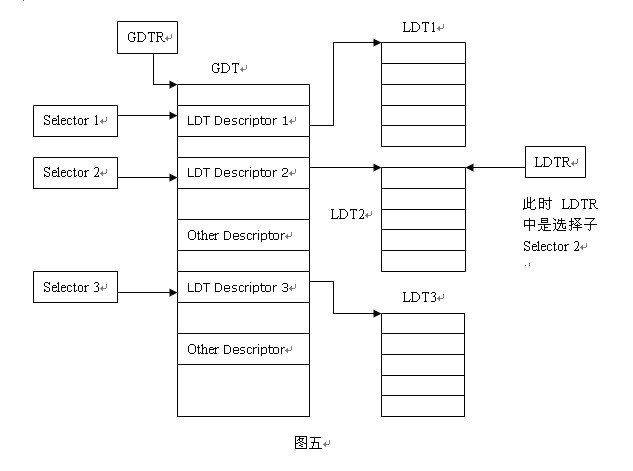
\includegraphics[width=15cm]{img/ldt0.png}
		\bottomcaption{LDT 布局}
	\end{figure}
	\subsection{TSS}
	在一个多任务环境中,当任务发生切换时,必须保存现场(比如通用寄存器,段寄存器,栈指针等)。为了保存被切换任务的状态,并且在下次执行它时恢复现场,每个任务都应当有一片内存区域,专门用于保存现场信息,x86默认支持这样一种任务状态段(Task State Segment)的格式。\\
	在创建一个任务的时候,我们要为这个任务创建TSS并填写其中的一些字段。\\
	\begin{itemize}
		\item 前一任务链接(TSS Back Link):TSS内偏移0处是前一个任务的TSS描述符的选择子。 当Call指令、中断或者异常造成任务切换,处理器会把旧任务的TSS选择子复制到新任务的TSS的Back Link字段中
		\item SS0,SS1,SS2和ESP0,ESP1,ESP2分别是0,1,2特权级堆栈的选择子和栈顶指针。这些内容应当由任务的创建者填写,且属于填写后一般不变的静态字段。
		\item CR3,指用户程序的页目录物理地址。供页表切换时使用。
		\item 偏移为0x20~0x5C的区域是处理器各个寄存器的快照部分,用于任务切换时保存现场。在一个多任务环境中,每次创建一个任务,内核至少要填写EIP,EFLAGS,ESP,CS,DS,SS,ES,FS和GS。
		\item LDT选择子是当前任务的LDT选择子,由内核填写,以指向当前任务的LDT。该信息由处理器在任务切换时使用,在任务运行期间保持不变。
		\item T(Debug Trap)位用于软件调试。在多任务环境中,如果T=1,则每次切换到该任务的时候,会引发一个调试异常中断(int 1).
		\item I/O位图基地址用来决定当前的任务是否可以访问特定的硬件端口。

	\end{itemize}
	和LDT一样,必须为每个TSS在GDT中创建对应的描述符。\\
	任务是不可重入的。就是说在多任务环境中,如果一个任务是当前任务,那么它可以切换到其他任务,但是不能从自己切换到自己。在TSS描述符中设置B位,并由处理器固件进行管理,可以防止这种情况的发生。\\

	\subsection{TCB}
	尽管不是处理器的要求,为了便于内核程序组织,我们额外还设计了TCB的数据结构。用于简要记录LDT,TSS在内核页表映射下的位置。\\
	为了表示程序运行状态, 增加State用+-1表示是否正在运行(相当于TSS的Busy位)
	在创建一个任务,需要使用比如程序的大小,加载的位置等等,当任务执行结束,还要依据这些信息来回收任务所占用的内存空间。\\
	\subsection{为高特权级使用的栈}
	如果在Y用户程序执行的过程中发生了由门发起的任务切换,那么就需要使用用户所提供的栈。毕竟这个新的任务在逻辑上还是隶属于用户程序。所以在分配内存的时候,需要为所有高于当前用户的特权级都设立一个栈。\\

\section{实验代码设计}
	\subsection{内存管理}
	比起实验五,这次加载的用户程序长度不定,内存加载逐渐变得动态了起来。为了管理低端2MB的内存空间,我们建立一个bitmap来记录哪些页已经被使用过了哪些还没有。分配内存的时候以此来遍历空闲页
	\begin{lstlisting}[language={[ANSI]C},keywordstyle=\color{blue!70},commentstyle=\color{red!50!green!50!blue!50},frame=shadowbox, rulesepcolor=\color{red!20!green!20!blue!20}]
#define page_map_len 64
u8 page_bit_map[page_map_len]=
				{0xff,0xff,0xff,0xff,0xff,0xff,0xff,0xff,			//低端都是土狼驻地地方
					0xff,0xff,0xff,0xff,0xff,0xff,0xff,0xff,
				0xff,0xff,0xff,0xff,0xff,0xff,0xff,0xff,
				0xff,0xff,0xff,0xff,0xff,0xff,0xff,0xff,
				0x55,0x55,0x55,0x55,0x55,0x55,0x55,0x55,
				0x00,0x00,0x00,0x00,0x00,0x00,0x00,0x00,
				0x00,0x00,0x00,0x00,0x00,0x00,0x00,0x00,
				0x00,0x00,0x00,0x00,0x00,0x00,0x00,0x00};

u32 allocate_a_4k_page(){
	for (int i=0; i<page_map_len<<3; ++i){
		if ( (page_bit_map[i>>3]&(1<<(i&0x7)))==0){
			page_bit_map[i>>3]^=1<<(i&0x7);
			return i<<12;
		}
	}
	simple_puts("Wrong On allocated page!", (3*80<<16)+0x8);
	return -1;
}
	\end{lstlisting}
	然后就需要实现在当前页目录下为某个线性地址分配页了。先由页目录找页表,再由页表找页。每一步不存在的页都需要进行分配。
	\begin{lstlisting}[language=={[x86masm]Assembler}keywordstyle=\color{blue!70},commentstyle=\color{red!50!green!50!blue!50},frame=shadowbox, rulesepcolor=\color{red!20!green!20!blue!20}]
alloc_inst_a_page:							;分配一个页,并安装在当前活动的
                                            ;层级分页结构中
                                            ;void alloc(页的线性地址)
											;如果存在就不分配了
		push eax
		push ebx
		push esi

		;check the exist of PageSheet
		mov esi, [esp+0x10]
		shr esi, 22
		shl esi, 2
		or esi, 0xfffff000
		test dword [esi], 0x01
		jnz .b1	

		;创建该线性地址所对应的页表 
        call allocate_a_4k_page            ;分配一个页做为页表 
        or eax,0x00000007
        mov [esi],eax   
	.b1:

		mov esi, [esp+0x10]
		shr esi, 12
		shl esi, 2
		or esi, 0xffc00000

		test dword[esi], 0x01
		jnz .b2

		call allocate_a_4k_page
		or eax, 0x07
		mov [esi], eax
	.b2:
		pop esi
		pop ebx
		pop eax

		ret
	\end{lstlisting}
	
	
	\subsection{加载用户程序}
	用户程序在加载的过程大概如下:
	\begin{itemize}
		\item 将当前页目录的前2GB清空,然后加载用户程序到0x0的线性地址。
		\item 申请TCB,TSS和LDT的地址空间,然后一边申请数据段,代码段和栈段,一边安装描述符到LDT和GDT
		\item 将剩余的空间安装完毕,申请新的页目录,然后拷贝当前内核页目录到新的地址。
	\end{itemize}
	\begin{lstlisting}[language={[ANSI]C},keywordstyle=\color{blue!70},commentstyle=\color{red!50!green!50!blue!50},frame=shadowbox, rulesepcolor=\color{red!20!green!20!blue!20}]
extern void Load_program(int sectors){
	Clean_partial_PDE();							//清理前2GB的页目录
	read_hard_disk_1(sectors,c_buf);
	u32 siz = *((u32*)c_buf); 
	u32 totsec=((siz+0x0fff)>>12)<<3;
	struct TCB *t = &tottcb[cnttcb++];
	u32 prog_addr=0;  						//用户程序的起始线性地址为0
	for (u32 i=0; i<totsec || i<80; ++i,prog_addr+=512){   // 至少分配10页给代码和GCC数据段
		alloc_inst_a_page(prog_addr);
		if ( i<totsec) read_hard_disk_1(sectors+i, prog_addr);
	}

	t->TSS_bas=TSS_array; TSS_array+=0x1000; // allocate 4KB/per tss,TSSarray指向全局的地址空间
	t->TSS_lim=103;

	alloc_inst_a_page(t->LDT_bas=prog_addr);			//分配一个页作LDT
	t->LDT_lim=-1;prog_addr+=0x1000;

	struct TSS *tssp = t->TSS_bas;
	tssp->CS=AddDescri_2_ldt(
		0x00000000,0x00000009,0x00c0f800, t
	)|0x3; // 建立代码段描述符并放入ldt中,返回段选择子,特权级设为3, 长度10页
	tssp->DS=tssp->ES=tssp->FS=tssp->GS=AddDescri_2_ldt(
		0x00000000,0x0000001A,0x00c0f200,t
	)|0x3;// 建立数据段描述符并放入ldt中,返回段选择子。特权级设为3 , 长度27页

	//将数据段作为用户任务的3特权级固有堆栈
	tssp->SS=tssp->DS;tssp->ESP=0x1b*0x1000;					//能不能不减4?
	
	//在用户任务的局部地址空间内创建0特权级堆栈,长度1页
	alloc_inst_a_page(prog_addr);
	tssp->SS0=AddDescri_2_ldt(
		prog_addr, 0x00000fff, 0x00409200,t					
	)|0x0; // ;设置选择子的特权级为0
	prog_addr+=0x1000;
	tssp->ESP0=0x00001000;							// bug, 真实地址==esp+ssbase!!!!!! esp0=0xfff!!!!而不是prog_addr

	//在用户任务的局部地址空间内创建1特权级堆栈,长度1页
	alloc_inst_a_page(prog_addr);
	tssp->SS1=AddDescri_2_ldt(
		prog_addr, 0x00000fff, 0x0040b200,t			// why ???????
	)|0x1; // ;设置选择子的特权级为1
	prog_addr+=0x1000;
	tssp->ESP1=0x00001000;

	//在用户任务的局部地址空间内创建2特权级堆栈,长度1页
	alloc_inst_a_page(prog_addr);
	tssp->SS2=AddDescri_2_ldt(
		0x0, 0x00000fff, 0x0040d200,t
	)|0x2; // ;设置选择子的特权级为2
	prog_addr+=0x1000;
	tssp->ESP2=0x00001000;

	//;在GDT中登记LDT描述符,并填写到TCB,TSS中
	t->LDT_sel=tssp->LDTsel=AddDescri_2_gdt(
		t->LDT_bas, t->LDT_lim, 0x00408200
	);
	
	tssp->preTSS=0x0;tssp->IOmap=t->TSS_lim;
	tssp->T=0;

	//;在GDT中登记TSS描述符,并填写到TCB,
	t->TSS_sel=AddDescri_2_gdt(
		t->TSS_bas, t->TSS_lim, 0x00408900
	);
	
	//总共27页,全部分配完	多分配一页?
	for (;prog_addr<(0x1C<<12); prog_addr+=0x1000)
		alloc_inst_a_page(prog_addr);
	

	alloc_inst_a_page(0xffffe000);//分配一个页作页目录,由于还没有切换页表,对新页表的操作还需要在内核页表中进行,反正页目录和页表的US位为0,也不需要在用户空间里
	memcpy(0xffffe000,0xfffff000,0x1000);
	tssp->CR3 = Phyaddr(0xffffe000);
	tssp->EFLAG= getEFLAGS();
	tssp->EIP= *((u32*)(0x4));
//	*((*u32)(tssp->CR3+0x4*0x3ff)) =   prog_addr// 这一步不需要获取实际物理地址
	t->next_bas=prog_addr;
	t->state=0;
	

	append_to_tcb_link(t);
	// alloc_inst_a_page(prog_addr);	//分配一个页作页表
	// for (int i=0; i<1024; ++i)
	// 	*((u32*)(prog_addr+i*4))= start_addr+i*4096;  // 低端12位信息待定

}

	\end{lstlisting}
	而内核的程序由于已经在mbr.asm中安装完毕,则只需要申请一块TSS的空间并填写即可。

	\begin{lstlisting}[language={[ANSI]C},keywordstyle=\color{blue!70},commentstyle=\color{red!50!green!50!blue!50},frame=shadowbox, rulesepcolor=\color{red!20!green!20!blue!20}]
extern u16 Load_coreself(){			//返回TSS选择子
	TSS_array=tss_linear_address;  //所有的TSS空间都在内核的空间进行分配。
	struct TCB *t= &tottcb[cnttcb++];
	t->pre=0; t->state= 0xffff;t->next_bas=0x80100000;
	t->LDT_lim=0xffff;
	struct TSS *tssp=t->TSS_bas=TSS_array;
	t->TSS_lim= 103;
	// alloc_inst_a_page(t->TSS_bas);
	TSS_array+=0x1000;
	tssp->preTSS=0x0;tssp->CR3=getCR3();			//填入cr3
	tssp->LDTsel=tssp->T=0;tssp->IOmap=103;

	t->TSS_sel=AddDescri_2_gdt(
		t->TSS_bas, t->TSS_lim, 0x00408900			//制作TSS的描述符,指向TSS所在空间并安装到GDT中。
	);
	append_to_tcb_link(t);
	return t->TSS_sel;
}
	\end{lstlisting}
	\begin{lstlisting}[language={[ANSI]C},keywordstyle=\color{blue!70},commentstyle=\color{red!50!green!50!blue!50},frame=shadowbox, rulesepcolor=\color{red!20!green!20!blue!20}]
	\end{lstlisting}
	上面用到的安装GDT ,LDT,以及获取特殊寄存器的中间函数如下
	\begin{lstlisting}[language=={[x86masm]Assembler}keywordstyle=\color{blue!70},commentstyle=\color{red!50!green!50!blue!50},frame=shadowbox, rulesepcolor=\color{red!20!green!20!blue!20}]
AddDescri_2_ldt:				;AddDescri_2_ldt(bas, lim, attri, *tcb)
								; 返回选择子
		push ebx
		push ecx
		push edx
		push edi

		mov eax , [esp+0x14]
		mov ebx , [esp+0x18]
		mov ecx , [esp+0x1c]

		call flat_4gb_code_seg_sel:make_seg_descriptor

		mov edi , [esp+0x20]
											;gcc中的struct 会有对齐的情况,注意。
		mov ebx , [edi+0x0c]				;ldt base
		xor ecx, ecx
		mov cx , [edi+0x0a]					;ldt limit
		inc cx
		add ebx, ecx

		mov [ebx], eax						; bug ,swap of edx:eax
		mov [ebx+0x4], edx

		xor eax, eax
		mov ax, cx
		add cx, 7
		mov [edi+0xa], cx

		or ax ,0x4				;TI=1
		pop edi
		pop edx
		pop ecx
		pop ebx
		ret

AddDescri_2_gdt:				;AddDescri_2_gdt(bas,lim, attri)
								; 返回选择子

		push ebx
		push ecx
		push edx
		
		sgdt [pgdt]

		mov eax , [esp+0x10]
		mov ebx , [esp+0x14]
		mov ecx , [esp+0x18]
		call flat_4gb_code_seg_sel:make_seg_descriptor

		movzx ebx, word [pgdt]
		inc bx
		add ebx, [pgdt+2]
		
		mov [ebx], eax
		mov [ebx+4] , edx

		add word [pgdt] ,8
		
		lgdt [pgdt]
		xor eax, eax
		mov ax , [pgdt]
		shr ax , 3
		shl ax , 3

		pop edx
		pop ecx
		pop ebx
		ret

	\end{lstlisting}
	\begin{lstlisting}[language=={[x86masm]Assembler}keywordstyle=\color{blue!70},commentstyle=\color{red!50!green!50!blue!50},frame=shadowbox, rulesepcolor=\color{red!20!green!20!blue!20}]
		memcpy:
		push esi
		push edi
		push eax
		push ecx

		mov edi , [esp+0x14]
		mov esi , [esp+0x18]
		mov ecx , [esp+0x1c]

	.cpying:
		mov al, [esi]				; mov eax [esi] is error
		mov [edi] , al
		inc edi
		inc esi
		loop .cpying

		pop ecx
		pop eax
		pop edi
		pop esi
		ret

Phyaddr:
		push ebx
		mov ebx, [esp+0x8]
		shr ebx, 12
		shl ebx, 2
		or ebx, 0xffc00000
		mov eax, [ebx]
		and eax, 0xfffff000
		pop ebx

		ret 

getCR3:
		mov eax, cr3
		ret 
		global getEFLAGS
getEFLAGS:
		pushfd
		pop eax
		or eax, 0x00000200					; IF must be on 
		; and eax, 0xfffffdff					; IF try to be off ?
		ret 
Clean_partial_PDE:						;清空当前页目录的前半部分
										;(对应低2GB的局部地址空间) 
	pushad

		mov ebp, esp

		 
		mov ebx, 0xfffff000
		xor esi, esi
	.b1:
		mov dword [ebx+esi*4], 0x00000000
		inc esi
		cmp esi, 512
		jl .b1

		mov ebx, 0xfffffff8				;新页目录的缓存也要清掉
		mov dword [ebx], 0x00000000

		mov eax, cr3
		mov cr3, eax						;reflash TLB
	popad

	ret

	\end{lstlisting}
	\begin{lstlisting}[language=={[x86masm]Assembler}keywordstyle=\color{blue!70},commentstyle=\color{red!50!green!50!blue!50},frame=shadowbox, rulesepcolor=\color{red!20!green!20!blue!20}]

	\end{lstlisting}
	
	\subsection{安装系统调用中断}
	以下是供内存调用的系统调用中断。比实验五多了一个put\_char
	\begin{lstlisting}[language=={[x86masm]Assembler}keywordstyle=\color{blue!70},commentstyle=\color{red!50!green!50!blue!50},frame=shadowbox, rulesepcolor=\color{red!20!green!20!blue!20}]
sys_call_handler: 
									;5 system calls available
									; 切换ds
		push ds
		push eax
		mov ax , flat_4gb_data_seg_sel
		mov ds , ax
		pop eax

		cmp al, 0					;0  putchar , cl=char
		jne	.endhandle0
		push ecx
		call putchar
		add esp, 4
		jmp .endsyscall
	.endhandle0:

		cmp al, 1					;1	getchar , return al=getchar()
		jne	.endhandle1
		xor eax, eax
		sti							; ??? must be open to let keyboard handle to flush the keybuf
		call getchar
		cli
		jmp .endsyscall
		
	.endhandle1:
		cmp al, 2					;2	simple_puts , ebx=*str  , ecx=pos<<16+col
		jne	.endhandle2
		push ecx
		push ebx
		call simple_puts
		add esp , 8
		jmp .endsyscall
		
	.endhandle2:

		cmp al, 3					;3  simple_putchar , ebx= color_site,  cl = ch
		jne	.endhandle3
		push ebx
		push ecx
		call simple_putchar
		add esp, 8
		jmp .endsyscall
	.endhandle3:

		cmp al, 4					;4  clock() return BCD code 0x00HourMinSec
		jne	.endhandle4
		call curr_clock
		jmp .endsyscall
	.endhandle4:

		cmp al, 5					;5	clear screen()
		jne	.endsyscall

		call clear_screen

	.endsyscall:
		push eax
		mov ax , [esp+4]
		mov ds , ax
		pop eax
		add esp, 4
		iretd

	\end{lstlisting}
	然后是往IDT中添加中断,包括时钟中断和系统中断,由于用户特权级为3,那么中断门的DPL设为3
	\begin{lstlisting}[language=={[x86masm]Assembler}keywordstyle=\color{blue!70},commentstyle=\color{red!50!green!50!blue!50},frame=shadowbox, rulesepcolor=\color{red!20!green!20!blue!20}]
		mov eax, general_exeption_handler
		mov bx, flat_4gb_code_seg_sel
		mov cx, 0x8e00					;e表示中断,如果用任务门则0101B,且需要提供TSS选择子。
		call flat_4gb_code_seg_sel:make_gate_descriptor
		

		mov ebx, idt_linear_address
		xor esi, esi
   
   .idt0:
		mov [ebx+esi*8], eax
		mov [ebx+esi*8+4], edx
		inc esi
		cmp esi, 19
		jle .idt0

		mov eax, general_interrupt_handler
		mov bx, flat_4gb_code_seg_sel
		mov cx, 0x8e00
		call flat_4gb_code_seg_sel:make_gate_descriptor

		mov ebx, idt_linear_address
   .idt1:
		  mov [ebx+esi*8] , eax
		  mov [ebx+esi*8+4] , edx
		  inc esi
		  cmp esi , 255
		  jle .idt1
   
		  ; set clock interrupt

		set_up_Idescriptor rtm_0x70_interrupt_handle, 0x70 ,0xee00
		  ; set keyboard inter
		; set_up_Idescriptor keyboard_interrupt_handle,0x21 , 0xee00

		  ; set syscall 
		set_up_Idescriptor sys_call_handler, 0x11, 0xee00	;	dpl ->3 

	\end{lstlisting}
	\begin{lstlisting}[language=={[x86masm]Assembler}keywordstyle=\color{blue!70},commentstyle=\color{red!50!green!50!blue!50},frame=shadowbox, rulesepcolor=\color{red!20!green!20!blue!20}]
	\end{lstlisting}
	
	\subsection{扩展系统调用}

	为了能在用户程序中实现更加复杂的功能,考虑使用C语言.h和asm头文件交叉编译共同组成头文件。这样实现的功能就能够直接供C用户程序使用。
	\begin{lstlisting}[language={[ANSI]C},keywordstyle=\color{blue!70},commentstyle=\color{red!50!green!50!blue!50},frame=shadowbox, rulesepcolor=\color{red!20!green!20!blue!20}]
#ifndef STDCALL
#define STDCALL

typedef unsigned char u8;
typedef unsigned short u16;
typedef unsigned int u32;
typedef unsigned long long u64;
#define DelayTime 200000

extern void simple_putchar(u32 , u32);
extern u32 clock();

const int dx[4]={1, 1, -1,-1}, dy[4]={1,-1,1,-1};
int curx, cury=0,curd=0;
u32 randseed;

int Delay(int delayt){int j=0;for (int i=delayt; i--;)j+=i;return j;}
u32 rand(){return randseed=randseed*16807%0xffff;}

void c_block_stone(u32 BaseX, u32 BaseY, u32 Limx,u32 Limy,u32 color){
	curx=0;cury=0;
	for (int i=0; i<10000; ++i){
		simple_putchar('*', ((curx+BaseX)*80+cury+BaseY<<16)+color);
		Delay(DelayTime);
		simple_putchar(' ', ((curx+BaseX)*80+cury+BaseY<<16)+color);
		int nx=curx+dx[curd], ny=cury+dy[curd];
		if ( nx<0 || nx>=Limx) curd^=2;
		if ( ny<0 || ny>=Limy) curd^=1;
		curx+=dx[curd]; cury+= dy[curd];
	}
}

void c_snakewind(u32 BaseX, u32 BaseY, u32 Limx, u32 Limy){
	
	for (int step=(Limx<Limy ? Limx:Limy)>>1, i=0,cnt=0; i<step; ++i){
	// for (int i=0; i<2; ++i){
		for (int j=BaseY+i;j<(int)BaseY+Limy-i; ++j, cnt=(cnt+1)%15){
			simple_putchar('+',((BaseX+i)*80+j<<16)+4);
			Delay(DelayTime/10);
		}
		for (int j=BaseX+i; j<(int)(BaseX+Limx-i); ++j,cnt=(cnt+1)%15){
			simple_putchar('+',(j*80+BaseY+Limy-1-i<<16)+1);
			Delay(DelayTime/10);
		}
		for (int j=BaseY+Limy-i-1;j>=(int)(BaseY+i); --j,cnt=(cnt+1)%15){
			simple_putchar('+',((BaseX+Limx-1-i)*80+j<<16)+4);
			Delay(DelayTime/10);
		}
		for (int j=BaseX+Limx-i-1; j>=(int)(BaseX+i); --j,cnt=(cnt+1)%15){   // bugs, lack of int and -1 will >=0
			simple_putchar('+',(j*80+BaseY+i<<16)+1);
			Delay(DelayTime/10);
		}
	}
	for (int i=0; i<Limx; ++i)
		for (int j=0; j<Limy; ++j){
			simple_putchar(' ', ((i+BaseX)*80+j+BaseY<<16)+0x0);
			Delay(DelayTime/20);
		}
}

#define SNAKELEN 20
const int vdx[4]={0,1,0,-1}, vdy[4]={1,0,-1,0};
void c_snakerand(u32 BaseX, u32 BaseY,  u32 Limx, u32 Limy,const u8 *info, u32 color){
	randseed=(clock()+info[0]+info[1])|1;
	u8 x[SNAKELEN+1], y[SNAKELEN+1];
	for (int i=1; i<=SNAKELEN; ++i)x[i]=(i-1)/Limy, y[i]=(i-1)%Limy;
	for (int i=SNAKELEN;i; --i)
		simple_putchar(info[i-1], ((x[i]+BaseX)*80+y[i]+BaseY<<16)+color);
	for (u8 cnt=0,d=rand()%4;;++cnt){
		if ( cnt%6==0) d=rand()%4;
		for(x[0]=x[1]+vdx[d], y[0]= y[1]+vdy[d]; x[0]>=Limx || y[0]>=Limy; x[0]=x[1]+vdx[d], y[0]= y[1]+vdy[d])
			d=(d+1)%4;
		simple_putchar(' ',((x[SNAKELEN]+BaseX)*80+BaseY+y[SNAKELEN]<<16));
		for (int i=SNAKELEN;i; --i){
			x[i]=x[i-1]; y[i]=y[i-1];
			simple_putchar(info[i-1], ((x[i]+BaseX)*80+y[i]+BaseY<<16)+color);
		}
		Delay(DelayTime/3);
	}
}
#endif

	\end{lstlisting}
	
	\begin{lstlisting}[language=={[x86masm]Assembler}keywordstyle=\color{blue!70},commentstyle=\color{red!50!green!50!blue!50},frame=shadowbox, rulesepcolor=\color{red!20!green!20!blue!20}]
	\end{lstlisting}

	\subsection{时钟中断控制任务切换}
	当发生时钟中断时,需要从TCB链表中找出当前正在运行和未被运行的程序,对调程序运行状态之后,利用jmp far发起任务切换
	\begin{lstlisting}[language={[ANSI]C},keywordstyle=\color{blue!70},commentstyle=\color{red!50!green!50!blue!50},frame=shadowbox, rulesepcolor=\color{red!20!green!20!blue!20}]
extern u32 c_rtm_0x70_interrupt_handle(){
	// Out(0xa0, 0x20); Out(0x20, 0x20);
	// Out(0x70, 0x0c); In(0x71);

	buf[0] = message_cyc[curcyc++];buf[1]=0;
	curcyc&=3;
	simple_puts(buf, (24*80+79<<16) + 4);
	show_current_clock();
	if ( TCBHeader->pre ==0)return -1;
	struct TCB *curact=TCBHeader;
	while ( curact->pre) curact= curact->pre;
	curact->state=0;
	curact->pre=TCBHeader;TCBHeader=TCBHeader->pre;
	curact=curact->pre;
	curact->pre=0;curact->state=0xffFF;
	return curact;
}
	\end{lstlisting}
	
	\begin{lstlisting}[language=={[x86masm]Assembler}keywordstyle=\color{blue!70},commentstyle=\color{red!50!green!50!blue!50},frame=shadowbox, rulesepcolor=\color{red!20!green!20!blue!20}]
		rtm_0x70_interrupt_handle:
		sti
		cli									;只是为了方便设断点
		push ds
		push eax
		mov ax , flat_4gb_data_seg_sel
		mov ds , ax
		pop eax

		pushad
		mov al,0x20                        ;中断结束命令EOI
		out 0xa0,al                        ;向8259A从片发送
		out 0x20,al                        ;向8259A主片发送

		mov al,0x0c                        ;寄存器C的索引。且开放NMI
		out 0x70,al
		in al,0x71                         ;读一下RTC的寄存器C,否则只发生一次中断
										;此处不考虑闹钟和周期性中断的情况
		call c_rtm_0x70_interrupt_handle
											; C语言完成任务切换, 并返回下一个任务TCB指针
		cmp eax, 0xffffffff
		je .noxchg
		jmp far  [eax+0x14]				; u32 TSS_bas ; u16 TSS_sel
	.noxchg:
		popad

		push eax
		mov ax , [esp+4]
		mov ds , ax
		pop eax
		add esp, 4
		iretd

	\end{lstlisting}
	
	\subsection{四个用户程序实现}

	四个用户程序结构大概类似,都是一个不同的系统调用。分别在4个象限显示信息。
	\begin{lstlisting}[language={[ANSI]C},keywordstyle=\color{blue!70},commentstyle=\color{red!50!green!50!blue!50},frame=shadowbox, rulesepcolor=\color{red!20!green!20!blue!20}]
// user0
#include "syscall.h"

extern void cstart(){
	while (1)	c_block_stone(0,0, 13, 40,7);
}

// user 1
#include "syscall.h"

extern void cstart(){
	while (1)	c_snakewind(0,40, 13, 40);
}


// user2 
#include "syscall.h"

const u8 info[SNAKELEN+1]="OS in protect MODE---";
extern void cstart(){
	while ( 1) c_snakerand(13,0,12,40, info, 0xe);
}

//user3
#include "syscall.h"

const u8 info[SNAKELEN+1]="17341038 fuchang's***";
extern void cstart(){
	while (1)	c_snakerand(13, 40, 12,40, info, 0xa);
}
	\end{lstlisting}

	\begin{lstlisting}[language=={[x86masm]Assembler}keywordstyle=\color{blue!70},commentstyle=\color{red!50!green!50!blue!50},frame=shadowbox, rulesepcolor=\color{red!20!green!20!blue!20}]
			[bits 32]
			program_length dd prog_end-$$
			entry_point dd cstart

extern cstart
%include "trash_syscall.inc"
global _start
_start:
	jmp _start

		; mov al, 4			; clear _screen
		; int 0x11
		; call user_main


;---------------
[section .data]
	sign db 'this is data end'
	prog_end:

	\end{lstlisting}
	


\section{实验结果及分析}
	\begin{figure}[htbp]
		\centering
		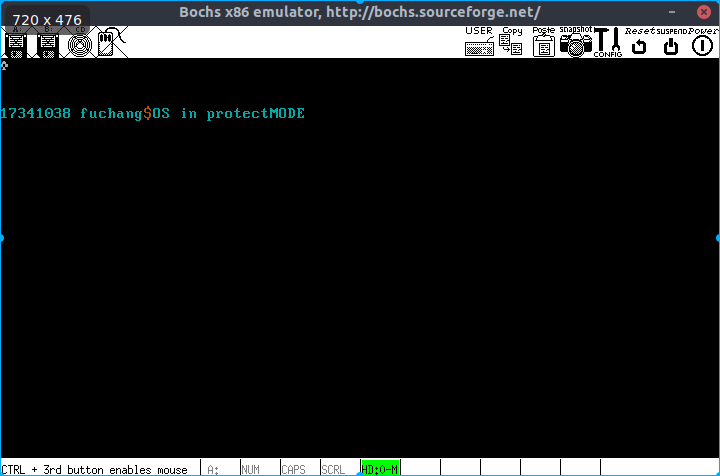
\includegraphics[width=15cm]{img/1.png}
		\bottomcaption{时钟中断正式开启,在内核显示个人信息}
	\end{figure}
	\begin{figure}[htbp]
		\centering
		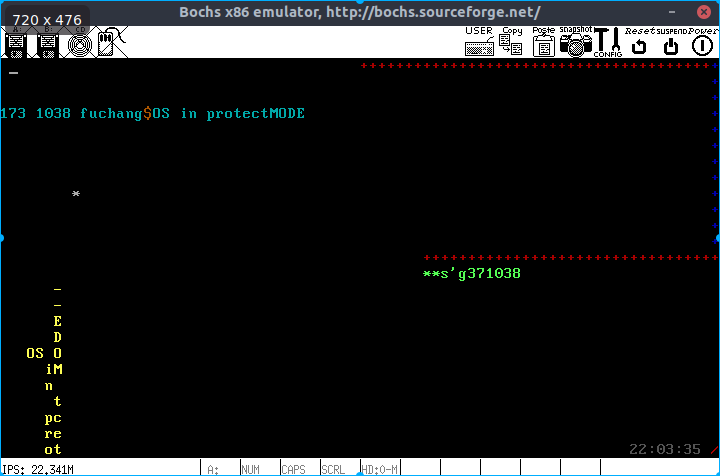
\includegraphics[width=15cm]{img/2.png}
		\bottomcaption{执行过程中的截图1,四个象限分别是弹球、环绕蛇和标识个人信息的随机游走蛇}
	\end{figure}
	\begin{figure}[htbp]
		\centering
		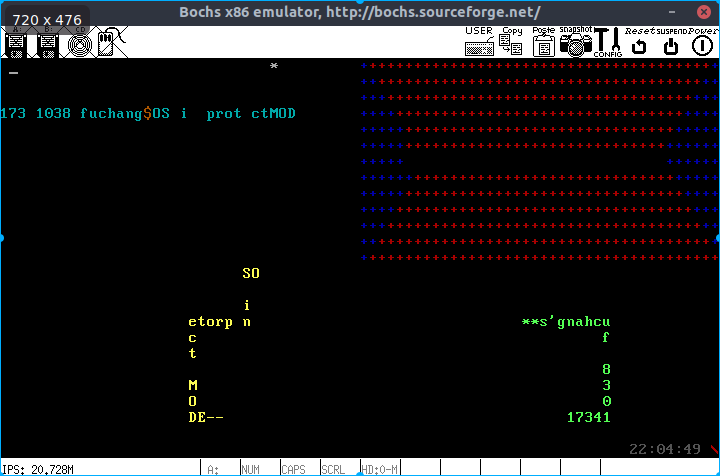
\includegraphics[width=15cm]{img/3.png}
		\bottomcaption{执行过程中的截图2,四个象限分别是弹球、环绕蛇和标识个人信息的随机游走蛇}
	\end{figure}
	如上图,时钟显示和风火轮照常显示。
	

\section{实验总结}
	这次实验比起前,更多的利用了TSS和LDT的功能。这两块的内容的设计非常繁琐,特别是TSS,稍有
\bibliographystyle{plain}
\bibliography{ref}

\clearpage



\end{document}
